\chapter{Big Bang Nucleosynthesis}\label{chap:bbn}

As discussed breifly in the Introduction, Big Bang Nucleosynthesis is a useful probe of new physics. In particular, new light states thermally coupled to the SM plasma can affect the synthesis of the primordial elements. While we are mostly interested in constraining MeV-scale dark matter particles, our analysis applies more generally to any additional BSM particles that are in thermal equilibrium with the SM during BBN and with a mass in the MeV range. This includes dark matter particles and mediators with the dark sector. In practice, this equilibrium should be maintained at temperatures below that of neutrino decoupling $T_\nu^{\rm dec} \sim 2\,\text{MeV}$~\cite{Dolgov:2002wy}. The requirement of being in thermal contact at least prior to neutrino decoupling restricts the couplings and masses of the particles we are able to constrain. For the case of weakly-interacting, stable, thermal BSM particles (WIMPs), it is well known that annihilation interactions with the SM plasma will decouple from chemical equilibrium at $T \sim m/20$~\cite{Kolb:1990vq}. Hence, our analysis will apply to thermal WIMPs with $m \lesssim 20\, T_\nu ^{\rm dec} \sim 40\,\text{MeV}$. In the case of unstable particles that decay into SM species, they will be in thermal equilibrium with the SM plasma during BBN, provided that their lifetime is $\tau \lesssim 0.1 \,\text{s}$. In other words, the lifetime should be shorter than the age of the Universe at the time of neutrino decoupling. Our analysis will constrain particles that efficiently annihilate or decay into neutrinos or electrons/photons prior and during neutrino decoupling. This is the case if the interaction rate is larger than the expansion rate $H$ at neutrino decoupling:
\begin{align}
    \Gamma \gtrsim H|_{T = T_\nu^{\rm dec}} \simeq 10 \,\text{s}^{-1}.
\end{align}
Throughout the text we will denote a generic BSM particle as $\chi$. For a particle that annihilates into SM species, the rate is $\Gamma \sim n\left<\sigma v \right> \sim g_\chi^2 g_{\rm SM}^2T^3/(16 \pi m_\chi^2)$ and our analysis will generally be sensitive to
\begin{align}\label{eq:Annihilation}
\text{Stable Particles with} \qquad  \,\,\,\,\,
    \sqrt{g_\chi g_{\rm SM}} \gtrsim  2\times 10^{-5} \sqrt{\frac{m_\chi}{\text{MeV}}} \qquad\qquad\qquad \,\,\,\,\,\,\,\,\,\, \text{and} \qquad m_\chi \lesssim 20\,\text{MeV}\,,
\end{align}
where $g_\chi$ and $g_{\rm SM}$ are coupling constants. If the $\chi$ particle is unstable, then $\Gamma \sim g_{\rm SM}^2m_\chi /(4\pi) \, K_{1}(m_\chi/T_{\nu}^{\rm dec})$ -- $K_{1}$ being a modified Bessel function of the first kind -- and our analysis will constrain
\begin{align}\label{eq:Decay}
\text{Unstable Particles with} \qquad 
    g_{\rm SM} \gtrsim  5\times 10^{-10} \sqrt{\frac{m_\chi}{\text{MeV}}}\left(1+ \sqrt{\frac{\text{MeV}}{m_\chi}} \right) \qquad \text{and} \qquad m_\chi \lesssim 20\,\text{MeV}.
\end{align}
In summary, the bounds we derive in this paper will generically constrain MeV-scale particles coupled to the SM bath with couplings $ \gtrsim 10^{-5}$ if they are stable\footnote{This would cover well the case of thermal dark matter, for which $\sqrt{g_\chi g_{\rm SM}} \sim 10^{-3} \sqrt{\frac{m_\chi}{10\,\text{MeV}}} \sqrt[4]{\frac{\left<\sigma v\right>}{3\times 10^{-26}\,\text{cm}^3/s} }$.} and with couplings as small as $10^{-9}$ if they are unstable. Note that our bounds will apply even if these unstable BSM particles decay into other BSM states, under the condition that they possess couplings $\gtrsim 10^{-9}$ to SM particles.

\section{Cosmology with Light WIMPs}
The implications of light, thermally coupled BSM particles with the SM plasma at temperatures $T \sim 1 \,\text{MeV}$ are twofold~\cite{Kolb:1986nf}: \textit{i)} they contribute to the expansion rate of the early Universe and \textit{ii)} they release entropy into the plasma.
In addition, if the new particles interact with both neutrinos and electrons/photons, they would efficiently delay the process of neutrino decoupling~\cite{Serpico:2004nm,Escudero:2018mvt}.

%%%%%%%%%%%%%%%%%%%%%%%%%%%%%%%%%%%%%%%%%%%%%%%%%%%%%%
\subsection{Temperature Evolution and Universe's Expansion}\label{sec:earlyUniverse_method}
%%%%%%%%%%%%%%%%%%%%%%%%%%%%%%%%%%%%%%%%%%%%%%%%%%%%%%

In order to accurately account for such effects we follow~\cite{Escudero:2018mvt} and assume that all relevant species can be described by thermal distributions and characterized by a temperature $T_i$. We then calculate the evolution of neutrino decoupling in terms of the temperature of the neutrinos and electromagnetic components of the plasma. For the details, methodology and differential equations governing this evolution, see Appendix \ref{sec:evo}. By solving the relevant equations, we find all the key background evolution quantities as a function of time, scale factor and temperature. In addition, we evaluate the number of effective relativistic degrees of freedom $N_{\rm eff}$ as relevant for CMB observations,
\begin{align}\label{eq:Neff}
N_{\rm eff} \equiv \frac{8}{7}\left(\frac{11}{4} \right)^{4/3} \left( \frac{\rho_{\text{rad}}-\rho_\gamma}{\rho_\gamma}\right) = 3 \left(\frac{11}{4} \right)^{4/3} \left(\frac{T_\nu}{T_\gamma}\right)^4 \, ,
\end{align}


%%%%%%%%%%%%%%%%%%%%%%%%%%%%%%%%%%%%%%%%%%%%%%%%%%%%%%
\subsection{Nucleosynthesis in the Presence of Thermal BSM Particles}\label{sec:earlyUniverse_method}
%%%%%%%%%%%%%%%%%%%%%%%%%%%%%%%%%%%%%%%%%%%%%%%%%%%%%%

MeV-scale thermal relics affect the synthesis of the light elements, see e.g.~\cite{Kolb:1986nf,Serpico:2004nm,Boehm:2013jpa,Nollett:2013pwa,Nollett:2014lwa}. In this work, we have modified the publicly available state-of-the-art BBN code \texttt{PRIMAT}~\cite{Pitrou:2018cgg} to accommodate for the presence of light BSM particles in thermal equilibrium with the SM plasma. This is done by computing the background cosmology externally using \texttt{NUDEC\_BSM} \cite{Escudero:2018mvt,Escudero:2019new} and then passing on the relevant parameters\footnote{This includes the evolution as a function of time and scale factor of $T_\gamma$, $T_\nu$, $H$ and the residual entropy transfer between neutrinos and electrons as parametrized by $\mathcal{N}$ in \texttt{PRIMAT} \cite{Pitrou:2018cgg}.} to the section of \texttt{PRIMAT} that takes care of the nuclear reaction rates and the time evolution of nuclei abundances. We have explicitly verified that the differences in the primordial element abundances between the default version of \texttt{PRIMAT} and with the SM evolution as calculated in \cite{Escudero:2018mvt,Escudero:2019new} are below $0.1\,\%$, and hence one order of magnitude smaller than current observational errors. Our results agree quantitatively and qualitatively with previous studies~\cite{Kolb:1986nf,Serpico:2004nm,Boehm:2013jpa,Nollett:2013pwa,Nollett:2014lwa}\footnote{We agree particularly well with \cite{Nollett:2013pwa,Nollett:2014lwa}, see Appendix~\ref{app:ComparisonsLiterature}. } modulo differences we attribute to updated nuclear reaction rates and the fact that we account for non-instantaneous neutrino decoupling, see Appendix~\ref{app:ComparisonsLiterature} for details.

%%%%%%%%%%%%%%%%%%%%%%%%%%%%%%%%%%%%%%%%%%%%%%%%%%%%%%
\subsection{Cosmological Implications}\label{sec:earlyUniverse_method}
%%%%%%%%%%%%%%%%%%%%%%%%%%%%%%%%%%%%%%%%%%%%%%%%%%%%%%
In this section we review the main cosmological implications of light BSM particles in thermal equilibrium with the Standard Model plasma during neutrino decoupling and Big Bang Nucleosynthesis. The reader is referred to~\cite{Kolb:1986nf,Serpico:2004nm,Boehm:2013jpa,Nollett:2013pwa,Nollett:2014lwa} for previous and complementary discussions of the impact of such particles on BBN and the CMB and to~\cite{Sarkar:1995dd,Iocco:2008va,Pospelov:2010hj} for reviews on the role of BBN as a probe of physics beyond the Standard Model. 

\vspace{0.5cm}
\noindent\textbf{Cosmic Microwave Background -- Modifications to $\boldsymbol{N_{\rm eff}}$} 

\noindent Once neutrinos decouple from the SM plasma at $T_\nu^{\rm dec} \lesssim 2\,\text{MeV}$, a light, neutrinophilic BSM particle of mass $m_\chi \lesssim 20 \,\text{MeV}$ will annihilate/decay into neutrinos, which results in $\rho_\nu > \rho_\nu^{\rm SM}$ or equivalently $N_{\rm eff} >N_{\rm eff}^{\rm SM}$. Analogously, an electrophilic particle will dump energy into the electromagnetic sector of the plasma at temperatures $T < T_\nu^{\rm dec}$ and yield $N_{\rm eff} < N_{\rm eff}^{\rm SM}$. In the upper panel of Figure~\ref{fig:Cosmoimply}, we display the corresponding value of $N_{\rm eff}$ for neutrinophilic and electrophilic BSM particles in thermal equilibrium with the SM plasma as a function of their mass. The grey contours correspond to the $\pm\,2\sigma$ measurements by Planck (see below). With the sole exception of an electrophilic scalar particle, it is clear that regardless of what the spin and number of internal degrees of freedom of a given species are, Planck would set a lower bound on its mass.

\vspace{0.5cm}
\noindent\textbf{Big Bang Nucleosynthesis}

\noindent Light BSM particles in thermal equilibrium during BBN lead to three main effects on the cosmological evolution that impact the synthesis of the primordial elements. Firstly, additional species present in the early Universe will alter the expansion rate and therefore also the temperature-to-time relation. This is important because they will modify the time at which various weak and nuclear processes freeze-out, in particular the proton-to-neutron conversion and $p + n \leftrightarrow  D + \gamma$. Secondly, the presence of these particles can change the evolution of the neutrino-to-photon temperature ratio. This has relevant implications because this ratio enters the proton-to-neutron conversion rates. Finally, light species thermally coupled to the electromagnetic sector of the plasma will release entropy after nucleosynthesis and therefore dilute the number density of all nuclei for a given primordial baryon-to-photon ratio. The impact of the particles considered in this work on the primordial abundances of helium and deuterium is depicted in the middle and lower panels of Figure~\ref{fig:Cosmoimply} and can be suitably categorised into three mass regions:
\newpage

\begin{enumerate}[leftmargin=0.7cm,itemsep=20pt]
    \item[\textbf{A.}] $\boldsymbol{m_\chi \lesssim 0.05 \, \mathrm{MeV}}$ \\ Very light neutrinophilic particles simply contribute to the expansion rate of the Universe during BBN, and do not alter the baryon-to-photon ratio. As such, they simply shorten the timescales on which the weak and nuclear processes freeze out, increasing both $Y_{\mathrm{P}}$ -- which is approximately proportional to the neutron-to-proton ratio at $T \sim 0.07 \, \mathrm{MeV}$ \cite{Sarkar:1995dd,Iocco:2008va,Pospelov:2010hj} -- and $\mathrm{D}/\mathrm{H}|_{\mathrm{P}}$ relative to the SM. Whilst very light electrophilic particles contribute to the expansion rate, which increases the value of $Y_{\mathrm{P}}$, they also release substantial amounts of entropy into the electromagnetic plasma \emph{after} nucleosynthesis. This acts to dilute number of baryons per photon and hence leads to a smaller value of $\mathrm{D}/\mathrm{H}|_{\mathrm{P}}$ than in the SM (since $\mathrm{D}/\mathrm{H}|_{\mathrm{P}} \propto \Omega_{\mathrm{b}}h^2$).
    
    \item[\textbf{B.}] $\boldsymbol{0.5 \, \mathrm{MeV} \lesssim m_\chi \lesssim 10 \, \mathrm{MeV}}$ \\ Electrophilic particles in this region lead to a smaller energy density of the Universe during nucleosynthesis and again to entropy release. This leads to lower values for both $Y_{\mathrm{P}}$ and $\mathrm{D}/\mathrm{H}|_{\mathrm{P}}$ as is seen in the lower two panels of Figure \ref{fig:Cosmoimply}. For neutrinophilic particles on the other hand, there is a larger energy density than in the SM, and hence a larger expansion rate. This leads to larger values for both $Y_{\mathrm{P}}$ and $\mathrm{D}/\mathrm{H}|_{\mathrm{P}}$ for a given $\Omega_{\rm b} h^2$.
    
    \item[\textbf{C.}] $\boldsymbol{m_\chi \gtrsim 30 \, \mathrm{MeV}}$ \\ In this region of masses the energy density of the particles at the time of nucleosynthesis is negligible since their number density is Boltzmann suppressed. As such, one recovers the SM predictions for the primordial element abundances.
\end{enumerate}

\noindent Of course, the abundances of other light elements like ${}^3\text{He}$ or ${}^{7}\text{Li}$ are also affected by the presence of light thermal BSM particles. However, such abundances are not typically used as cosmological probes~\cite{pdg}, and therefore we do not use them in this work. The interested reader is referred to Appendix~\ref{app:cosmo_imp_other} for the effect of different types of thermal BSM particles on these abundances. 

\vspace{1cm}
\noindent\textbf{Expectations}

\noindent From Figure~\ref{fig:Cosmoimply} we notice that thermal species of mass $m_\chi \lesssim 0.4-3\,\text{MeV}$ will be ruled out by current $Y_{\rm P}$ measurements. Note that $Y_{\rm P}$ is only logarithmically dependent upon the baryon energy density $\Omega_{\mathrm{b}}h^2$. One might also expect current ${\rm D/H}|_{\rm P}$ measurements to set stringent constraints on the mass of various BSM particles; about $m_\chi \lesssim 3-10\,\text{MeV}$. However, note that the ${\rm D/H}|_{\rm P}$ predictions are shown for a fixed value of $\Omega_{\mathrm{b}} h^2$ and ${\rm D/H}|_{\rm P} \propto \Omega_{\mathrm{b}} h^2$, thus deuterium measurements will only yield constraints provided that $\Omega_{\mathrm{b}} h^2$ is inferred from CMB observations or in conjunction with $Y_{\rm P}$ measurements.

\begin{figure}[h]
    \centering
    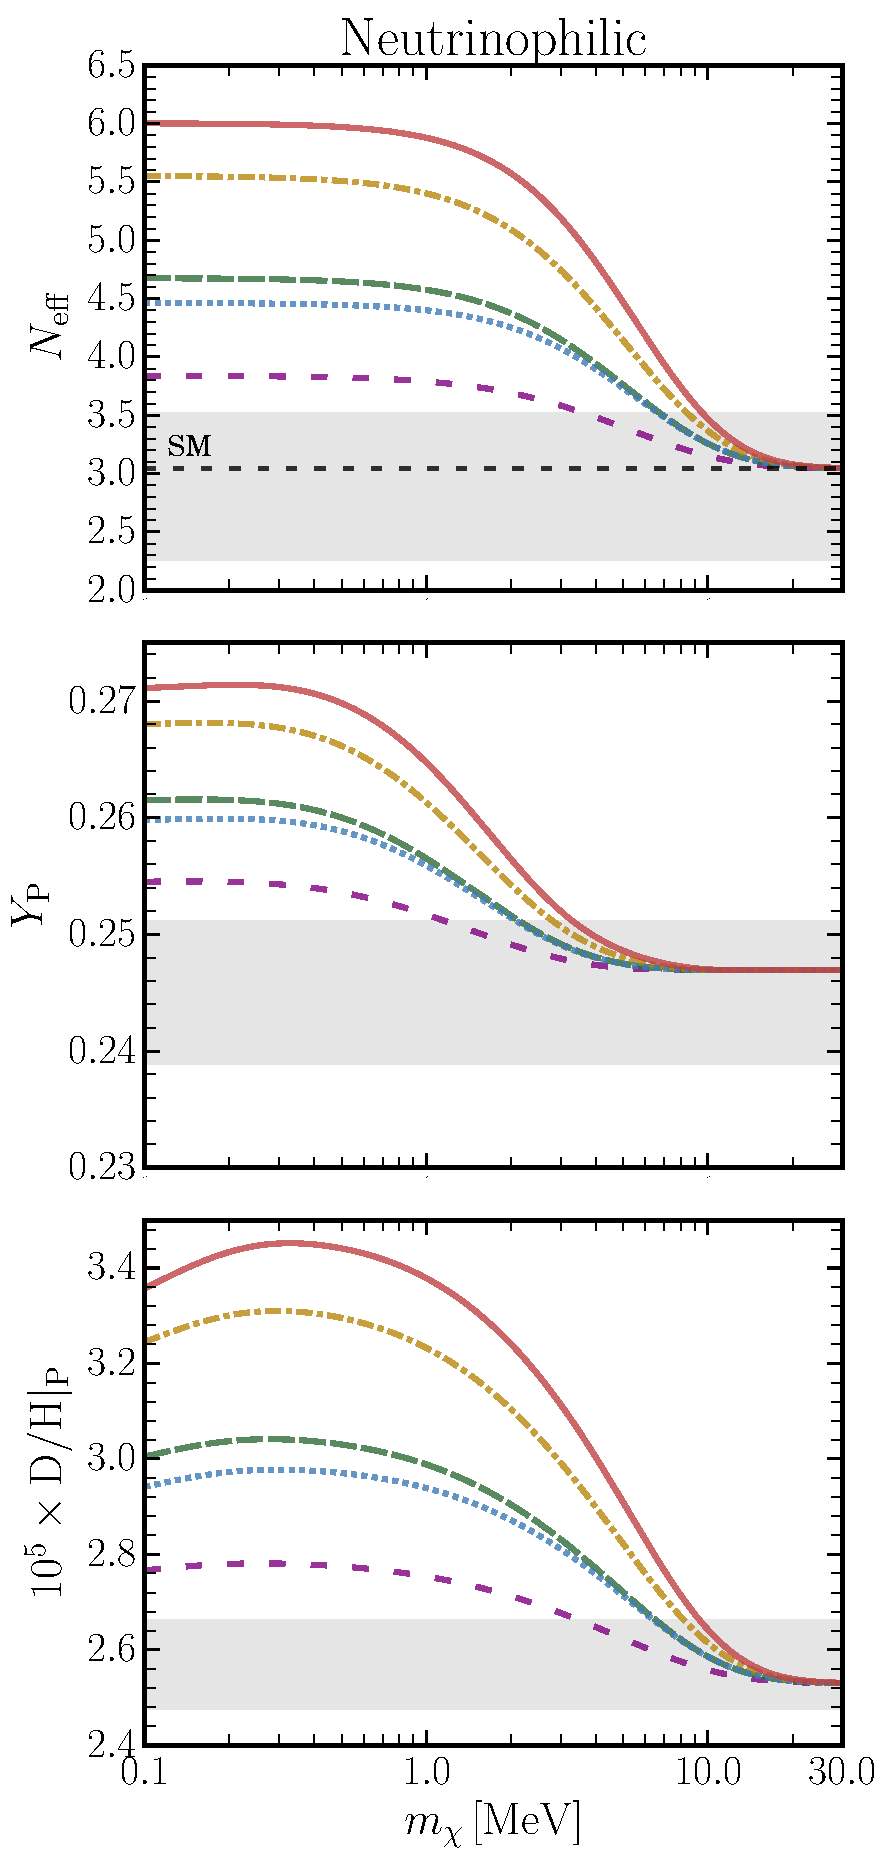
\includegraphics[width=0.45\textwidth]{figures/Nu_abundance_plot.pdf} \qquad
    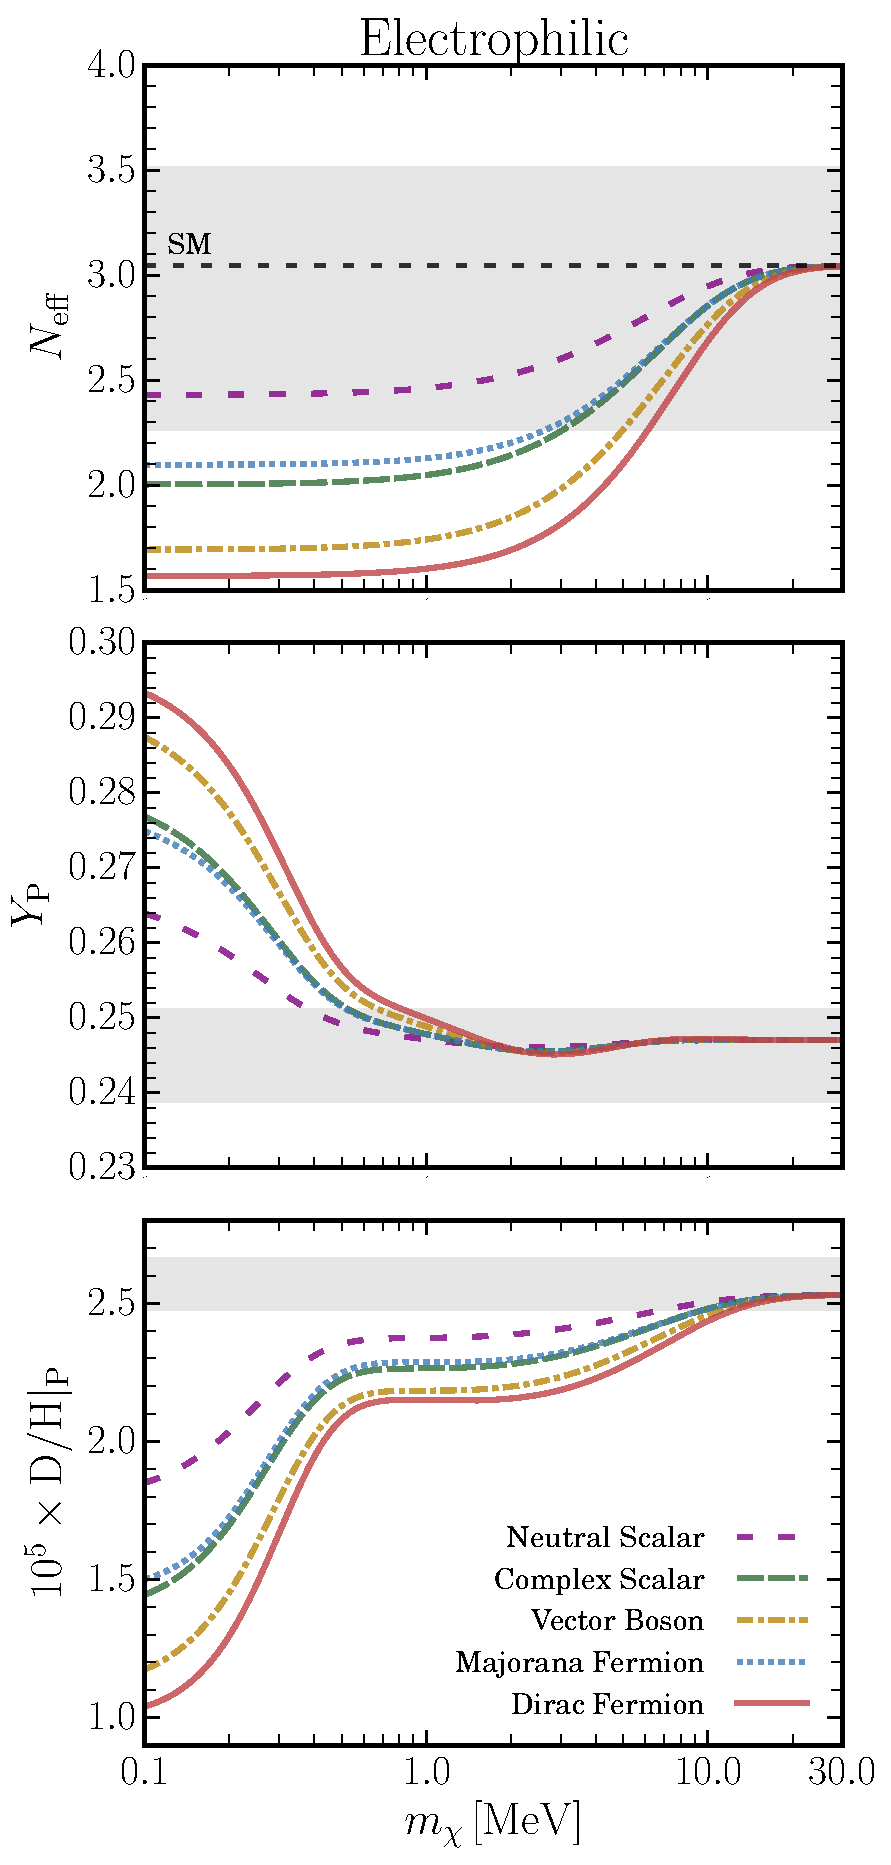
\includegraphics[width=0.45\textwidth]{figures/EE_abundance_plot.pdf}\vspace{-0.2cm}
    \caption{Cosmological impact of light BSM particles in thermal equilibrium with the SM plasma as a function of their mass $m_\chi$. The \textit{left/right panel} corresponds to neutrinophilic/electrophilic particles. \textit{Upper panels:} The number of effective relativistic neutrino species $N_{\rm eff}$ as relevant for CMB observations. \textit{Middle panels:} Primordial helium abundance $Y_{\rm P}$. \textit{Lower panels:} Primordial deuterium abundance ${\rm D/H}|_{\rm P}$. The $Y_{\rm P}$ and ${\rm D/H}|_{\rm P}$ predictions are computed with $\Omega_{\mathrm{b}} h^2 = 0.021875$ and $\tau_n = 879.5\,\text{s}$. The grey contours correspond to the mean $\pm \, 2\sigma$ measurements that enter our BBN and Planck data analyses, see Eqs.~\eqref{eq:chiBBN},~\eqref{eq:chi2_CMB}  and~\eqref{eq:CovarianceForm}.}
    \label{fig:Cosmoimply}
\end{figure}
\clearpage
\section{Cosmological Data and Analysis}\label{sec:current_data_analyis}
%%%%%%%%%%%%%%%%%%%%%%%%%%%%%%%%%%%%%%%%%%%%%%%%%%%%%%
\vspace{-0.05 cm}

In order to set constraints on the masses of various BSM particles, we perform very conservative analyses using the latest determinations of the primordial element abundances and CMB observations by the Planck satellite as described below. Table~\ref{tab:analysis_summary} provides a summary of the main data sets used in each analysis. 


\begin{table}[t]
\begin{center}
{\def\arraystretch{1.1}
\resizebox{\textwidth}{!}{
\begin{tabular}{lll}
\hline\hline
\textbf{Analysis}  $\qquad$            	   & \textbf{Cosmological Data} $ \,\,\,$	& \textbf{Description} \\ \hline\hline
\multirow{2}{*}{BBN}    &  \multirow{2}{*}{($Y_{\rm P}$,\,\,${\rm D/H}|_{\rm P}$)} & Mean values and error bars as recommended by the PDG. \\
 & & Theoretical uncertainties in the predictions are accounted for. \\ \hline

\multirow{2}{*}{BBN+$\Omega_{\mathrm{b}} h^2$}   & \multirow{2}{*}{$(Y_{\rm P}$,\,\,${\rm D/H}|_{\rm P},\,\Omega_{\mathrm{b}} h^2$)} & Same as BBN but with $\Omega_{\mathrm{b}} h^2 = 0.02225 \pm 0.00066$ from CMB observations. \\
 & & This represents a conservative and model independent range for $\Omega_{\mathrm{b}} h^2$. \\ \hline

\multirow{2}{*}{Planck}  & \multirow{2}{*}{$(\Omega_{\mathrm{b}} h^2,\,N_{\rm eff},\,Y_{\rm P})$} & From the Planck2018-TTTEEE+lowE analysis. \\
 & & Assumes $\Lambda$CDM + varying $N_{\rm eff}$ and $Y_{\rm P}$. \\ \hline

\multirow{2}{*}{Planck+$H_0$}  & \multirow{2}{*}{$(\Omega_{\mathrm{b}} h^2,\,N_{\rm eff},\,Y_{\rm P})$} & From the Planck2018-TTTEEE+lowE+lensing+BAO+$H_0$ analysis. \\
 & & Assumes $\Lambda$CDM + varying $N_{\rm eff}$ and $Y_{\rm P}$. \\ \hline

\multirow{2}{*}{Planck+BBN} & $(\Omega_{\mathrm{b}} h^2,\,N_{\rm eff},\,Y_{\rm P}) +$ & Joint constraint from Planck 2018 CMB observations and $Y_{\rm P}$ and ${\rm D/H}|_{\rm P}$\\
 & $(Y_{\rm P}$,\,\,${\rm D/H}|_{\rm P})$ & determinations as recommended by the PDG. \\   \hline \hline
\end{tabular}}
}
\end{center}\vspace{-0.3cm}
\caption{Summary of the different baseline analyses carried out in this work in order to constrain light BSM particles in thermal equilibrium with the SM plasma during BBN. For each analysis, a likelihood is computed on a grid of $(\Omega_{\rm b} h^2,\,m_\chi)$. }\label{tab:analysis_summary}
\end{table}

%%%%%%%%%%%%%%%%%%%%%%%%%%%%%%%%%%%%%%%%%%%%%%%%%%%%%%
\subsection{Big Bang Nucleosynthesis}\label{sec:BBN_data}
%%%%%%%%%%%%%%%%%%%%%%%%%%%%%%%%%%%%%%%%%%%%%%%%%%%%%%

We use the PDG recommended means and error bars for the observed primordial abundances of helium and deuterium, which at $1\sigma$ read \cite{pdg}:
\begin{align}
Y_{\rm P} 	            &= 0.245 \pm 0.003 \label{eq:Yp}\, , \\
{\rm D/H}|_{\rm P}   	&= (2.569  \pm 0.027) \times 10^{-5} \label{eq:DH} \,.
\end{align}
These values are based on the analyses/measurements of~\cite{2017RMxAC..49..181P,Aver:2015iza,Izotov:2014fga} and~\cite{Cooke:2016rky,Balashev:2015hoe,2018MNRAS.477.5536Z,Riemer-Sorensen:2017pey} for helium and deuterium respectively. 
In addition to the observational uncertainties in $Y_{\rm P}$ and ${\rm D/H}|_{\rm P}$, we account for theoretical uncertainties in the predicted abundances arising from uncertainties in the neutron lifetime\footnote{Since we account for the uncertainty in the neutron lifetime, in all analyses presented in this work, we shall fix the neutron lifetime to the default value in \texttt{PRIMAT}: $\tau_n =  879.5\,\text{s}$. This value is compatible with the PDG within $1\sigma$, $\tau_n = 880.2\pm 1\,\text{s}$~\cite{pdg}. Choosing $\tau_n = 880.2\,\text{s}$ will not alter any of the results presented in this study.} and various nuclear reaction rates. These are given by~\cite{Pitrou:2018cgg}:
\begin{align}
\sigma(Y_{\rm P})^{\rm Theo} 	        		&= 0.00017 \,, \\
\sigma({\rm D/H}|_{\rm P} )^{\rm Theo}   	&= 0.036 \times 10^{-5} \label{eq:sigmaDH} \, .
\end{align}
Assuming Gaussian statistics and combining in quadrature the observational and theoretical errors, we define the following effective BBN $\chi^2$: 
\begin{align}\label{eq:chiBBN}
\chi_{\rm BBN}^2 = \frac{\left[Y_{\rm P} - Y_{\rm P}^{\rm Obs}\right]^2}{\sigma_{Y_{\rm P}}^2|{}^{\rm Theo} + \sigma_{Y_{\rm P}}^2|{}^{\rm Obs}} + \frac{\left[{\rm D/H}|_{\rm P} - {\rm D/H}|_{\rm P}^{\rm Obs}\right]^2}{\sigma_{{\rm D/H}|_{\rm P}}^2|{}^{\rm Theo} + \sigma_{{\rm D/H}|_{\rm P}}^2|{}^{\rm Obs}} \, ,
\end{align}
which we will use to quantify deviations from the observed primordial abundances due to the presence of the new particles in the thermal bath.


%%%%%%%%%%%%%%%%%%%%%%%%%%%%%%%%%%%%%%%%%%%%%%%%%%%%%%
\subsection{Cosmic Microwave Background: Planck 2018}\label{sec:CMB_data}
%%%%%%%%%%%%%%%%%%%%%%%%%%%%%%%%%%%%%%%%%%%%%%%%%%%%%%
CMB observations measure very precisely three parameters that are relevant for our analysis: $\Omega_{\mathrm{b}} h^2,\,N_{\rm eff},\,Y_{\rm P}$. The baryon abundance $\Omega_{\mathrm{b}} h^2$ is one of the 6 parameters in $\Lambda$CDM and Planck reports measurements on $\Omega_{\mathrm{b}} h^2$ with greater than $1\%$ accuracy. $N_{\rm eff}$ represents one of the most important cosmological parameters and the current accuracy by the Planck satellite on this parameter is $\mathcal{O}(10\,\%)$. $Y_{\rm P}$ is also constrained by CMB observations, albeit with error bars that are typically a factor of 6 - 7 larger than those inferred from blue compact galaxies \cite{pdg}, see Equation~\eqref{eq:Yp}.

In this work, we use the latest CMB observations by the Planck satellite to set constraints on the masses and interactions of various BSM particles. Since the disagreement between local~\cite{Riess:2019cxk} and CMB determinations of the Hubble constant~\cite{Aghanim:2018eyx} could potentially be attributed to additional contributions to $N_{\rm eff}$~\cite{Bernal:2016gxb,Verde:2019ivm}, we consider two data sets: \textit{i)} in which we consider the 2018 Planck baseline TTTEEE+lowE analysis and \textit{ii)} where we combine Planck CMB data with Baryon Acoustic Oscillation (BAO) measurements~\cite{Beutler:2011hx,Ross:2014qpa,Alam:2016hwk} and the local measurement of $H_0$ as reported by the SH0ES collaboration~\cite{Riess:2019cxk}. We shall call the former data set Planck and the latter Planck+$H_0$.  

We build a Gaussian likelihood for the relevant parameters:
\begin{align}\label{eq:chi2_CMB}
\chi_{\rm CMB}^2  = \left(\Theta - \Theta_{\rm Obs}\right)^T \,  \Sigma_{\rm CMB}^{-1} \,\left(\Theta - \Theta_{\rm Obs}\right)\, , \qquad \text{with} \qquad \Sigma_{\rm CMB} = \,
 \left(
\begin{array}{ccc}
\sigma_1^2 & \sigma_1 \sigma_2 \rho_{12} & \sigma_1 \sigma_3 \rho_{13}  \\
\sigma_1 \sigma_2 \rho_{12}     & \sigma_2^2 & \sigma_2 \sigma_3 \rho_{23} \\
\sigma_1 \sigma_3 \rho_{13}     & \sigma_2 \sigma_3 \rho_{23}        & \sigma_3^2 \\
\end{array}
\right) \,, 
\end{align}
where $\Theta = (\Omega_{\mathrm{b}} h^2,\,N_{\rm eff},\,Y_{\rm P})$ and

\vspace{8pt}
\begin{minipage}{0.5\textwidth}
\centering \textit{Planck 2018}
\begin{align}\label{eq:CovarianceForm}
(\Omega_{\mathrm{b}} h^2,\,N_{\rm eff},\,Y_{\rm P})|_{\rm Obs} &= (0.02225,\, 2.89,\, 0.246),\nonumber  \\
(\sigma_{1},\,\sigma_{2},\,\sigma_{3}) &= (0.00022,\, 0.31,\, 0.018), \nonumber  \\
(\rho_{12},\,\rho_{13},\,\rho_{23}) &= ( 0.40,\, 0.18,\, -0.69) \,,
\end{align}
\end{minipage}
\begin{minipage}{0.49\textwidth}
\centering \textit{Planck 2018+BAO+$H_0$}
\begin{align}%\label{eq:CovarianceForm_H0}
(\Omega_{\mathrm{b}} h^2,\,N_{\rm eff},\,Y_{\rm P})|_{\rm Obs} &= (0.02345,\, 3.36,\, 0.249), \nonumber  \\
(\sigma_{1},\,\sigma_{2},\,\sigma_{3}) &= (0.00025,\, 0.25,\, 0.020), \nonumber      \\
(\rho_{12},\,\rho_{13},\,\rho_{23}) &= (0.011,\, 0.50,\, -0.64) \,,
\end{align}
\end{minipage}
\vspace{0.2cm}

\noindent where the covariance matrix for the Planck 2018 analysis has been extracted from the Planck database~\cite{Aghanim:2018eyx,Aghanim:2019ame}. The covariance matrix for the Planck 2018+BAO+$H_0$ analysis was obtained by running a Markov-Chain-Monte-Carlo analysis using \texttt{CLASS}~\cite{Blas:2011rf,Lesgourgues:2011re} and \texttt{Monte Python}~\cite{Brinckmann:2018cvx,Audren:2012wb} with Planck 2018 data~\cite{Aghanim:2018eyx,Aghanim:2019ame}, various BAO measurements~\cite{Beutler:2011hx,Ross:2014qpa,Alam:2016hwk} and by including a Gaussian likelihood on $H_0$ from the results of~\cite{Riess:2019cxk}. Clearly, the main implication of including local measurements of $H_0$ in the fit is the upward shift on the reconstructed value of $N_{\rm eff}$ from $2.89$ to $3.36$. 
 

%%%%%%%%%%%%%%%%%%%%%%%%%%%%%%%%%%%%%%%%%%%%%%%%%%%%%%
\subsection{BBN+CMB Data Combinations}\label{sec:Statistics}
%%%%%%%%%%%%%%%%%%%%%%%%%%%%%%%%%%%%%%%%%%%%%%%%%%%%%%
Combining measurements of the primordial element abundances and CMB observations proves useful in constraining light thermal species coupled to the SM plasma.

In this work, we will combine BBN+CMB data in two ways: \textit{i)} by constructing a joint $\chi^2$ that is obtained by summing the individual Planck and BBN $\chi^2$'s as defined in Eqs.~\eqref{eq:chiBBN} and~\eqref{eq:chi2_CMB} (labelled BBN+Planck across the paper) and \textit{ii)} by adding to $\chi^2_{\rm BBN}$ a measurement of $\Omega_{\mathrm{b}} h^2 = 0.02225 \pm 0.00066$, which is to be regarded as a cosmological model-independent Planck determination of the baryon energy density\footnote{The value $\Omega_{\mathrm{b}} h^2 = 0.02225 \pm 0.00066$ has an error $4.4$ times larger than the one associated with $\Lambda\text{CDM}$ using Planck 2018 observations~\cite{Aghanim:2018eyx}, and furthermore it covers well the inferred value of $\Omega_{\mathrm{b}} h^2$ in a well-motivated 12-parameter extension of $\Lambda$CDM using different data sets~\cite{DiValentino:2016hlg,DiValentino:2017zyq}.} (we shall call this analysis BBN+$\Omega_{\mathrm{b}} h^2$). See Appendix~\ref{app:Omegab} for details.

%%%%%%%%%%%%%%%%%%%%%%%%%%%%%%%%%%%%%%%%%%%%%%%%%%%%%%
\subsection{Statistical Assessment}\label{sec:Statistics}
%%%%%%%%%%%%%%%%%%%%%%%%%%%%%%%%%%%%%%%%%%%%%%%%%%%%%%

For each of the scenarios considered, the quantities $\chi^2_{\mathrm{BBN}}$ and $\chi^2_{\mathrm{CMB}}$ are computed on a grid of $(\Omega_{\mathrm{b}} h^2,\,m_\chi)$ and subsequently marginalized over $\Omega_{\mathrm{b}} h^2$. Then, by comparing the marginalized 1-D $\chi^2 (m_\chi)$ with the minimum $\chi^2_{\rm min}$, we consider a scenario to be ruled out at $2\sigma$ when $\Delta \chi^2 \equiv \chi^2 - \chi^2_{\mathrm{min}} = 4$. The statistical compatibility of each ${\chi}^2_{\mathrm{min}}$ is estimated by computing its p-value, which is found to be acceptable in all cases presented in this work. This is as expected, given that BBN predictions and CMB observations are compatible with each other within the Standard Model.



\begin{figure}[t]
    \centering
    \hspace*{-0.2 cm}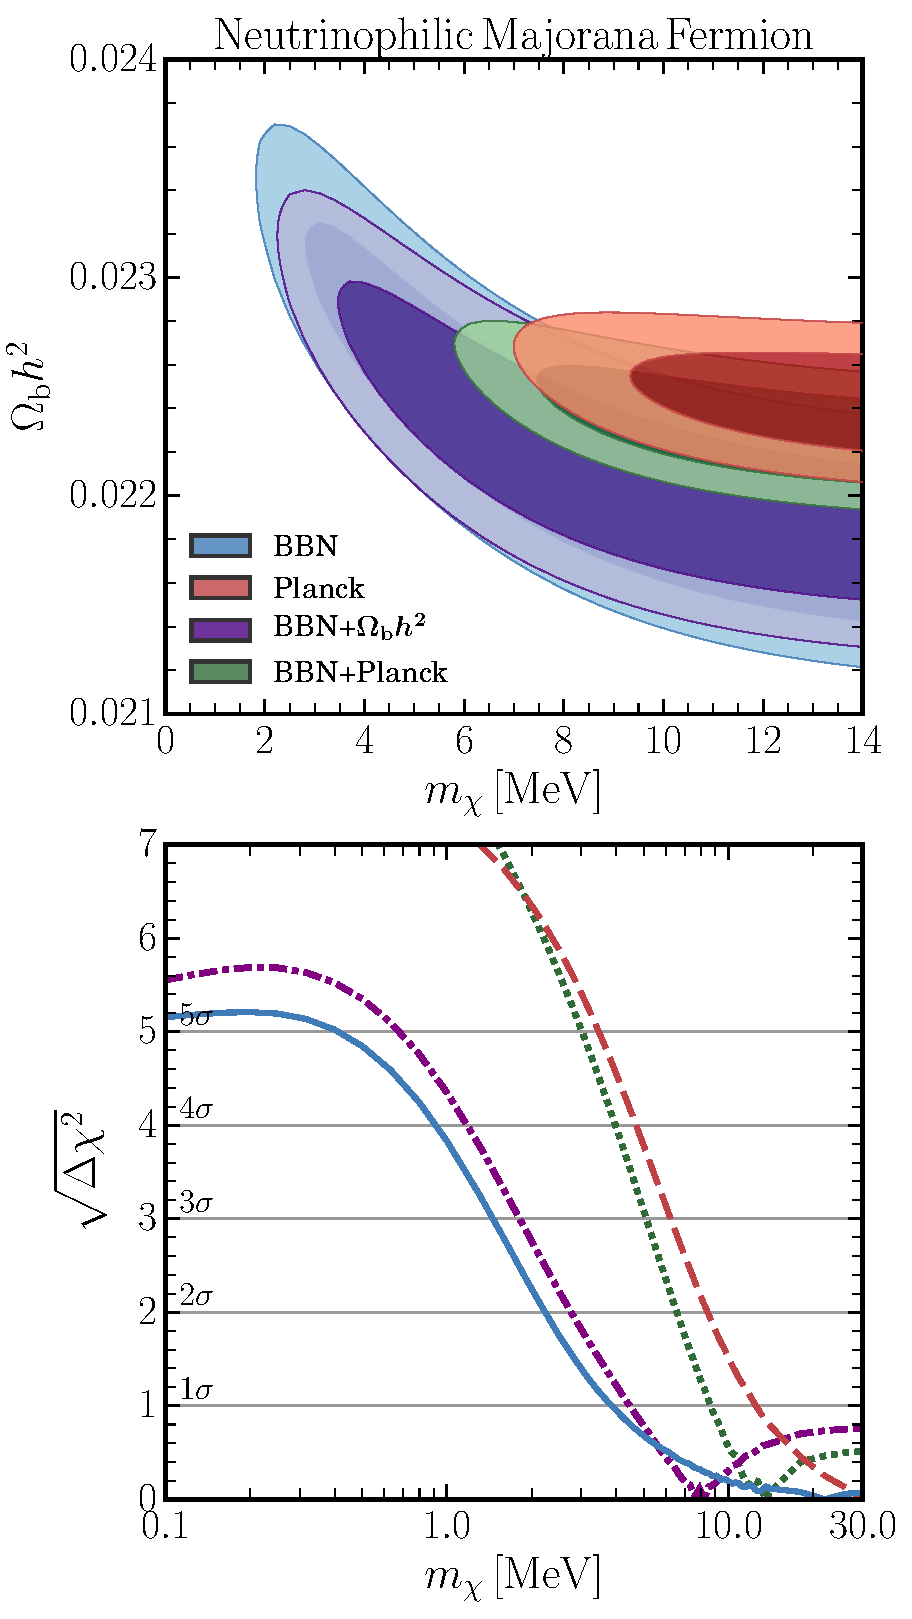
\includegraphics[width=0.45\textwidth]{figures/Nu_Maj_exclusion_and_deltachi.pdf} \quad
    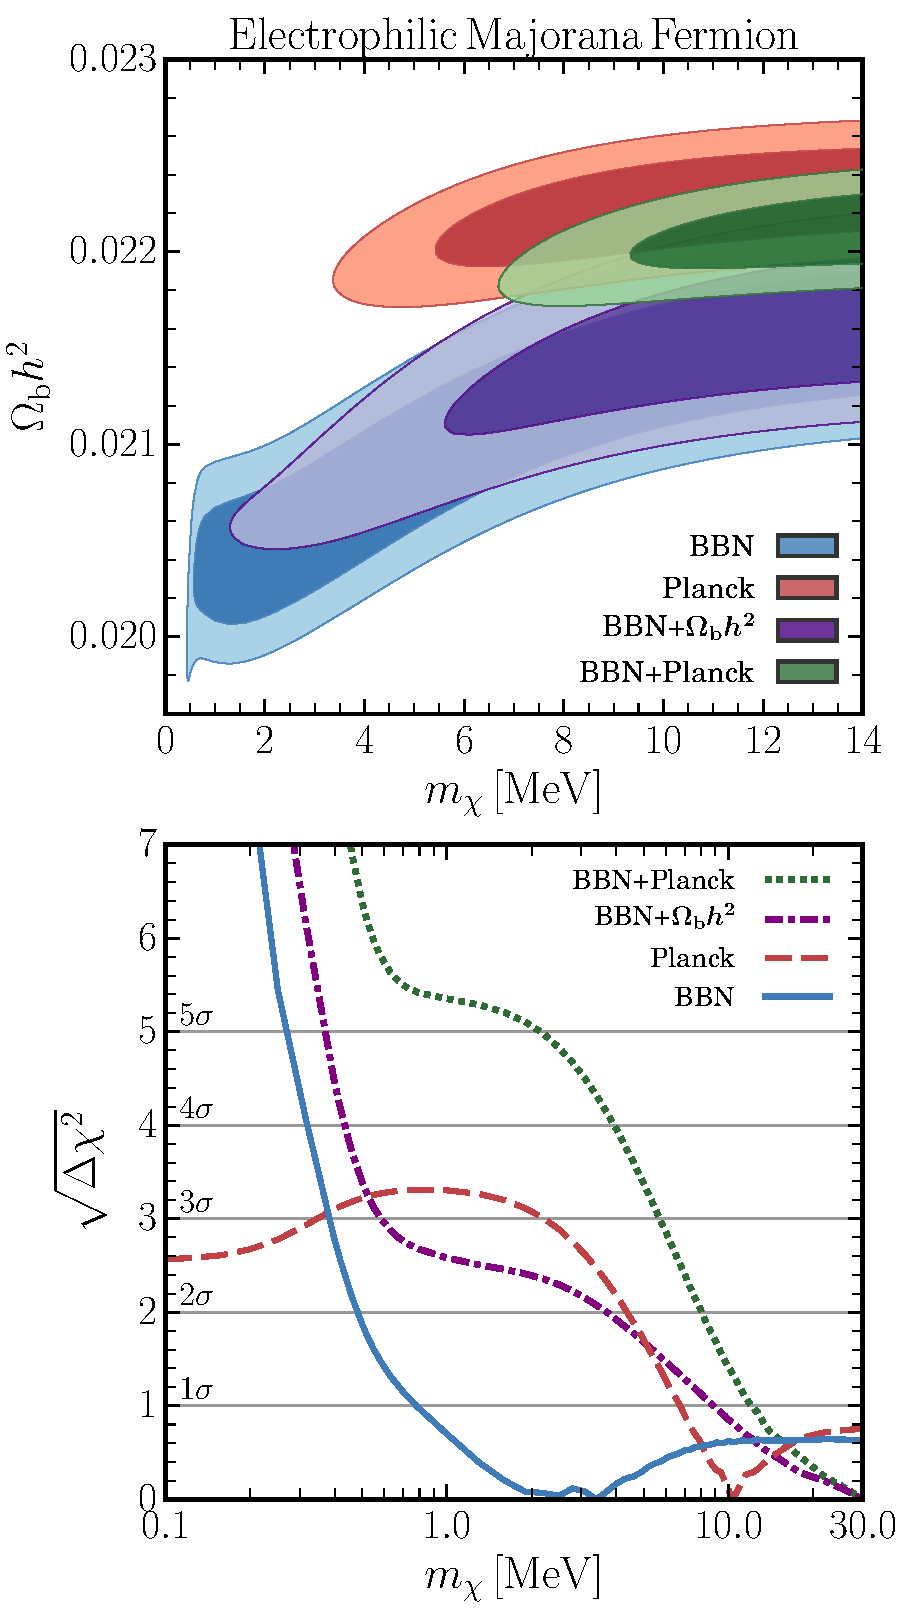
\includegraphics[width=0.45\textwidth]{figures/EE_Maj_exclusion_and_deltachi.pdf}
    \caption{\emph{Upper Panels:} Contour plots showing the $1\sigma$ and $2\sigma$ confidence intervals in the $(\Omega_{\mathrm{b}} h^2$,\,$m_\chi)$ plane for a Majorana fermion with mass $m_\chi$ in thermal equilibrium with the SM plasma. \emph{Lower Panels:} Marginalized $\Delta \chi^2$ as a function of $m_\chi$. Solid lines correspond to BBN constraints, dashed to Planck CMB 2018 observations, dash-dotted to the combination BBN+$\Omega_{\mathrm{b}}h^2$ and dotted to BBN+Planck. The \textit{left/right panel} corresponds to neutrinophilic/electrophilic particles.}
    \label{fig:Current_1-2D}
\end{figure}

\vspace{-0.3cm}

%%%%%%%%%%%%%%%%%%%%%%%%%%%%%%%%%%%%%%%%%%%%%%%%%%%%%%
\section{Current Cosmological Constraints}\label{sec:results}
%%%%%%%%%%%%%%%%%%%%%%%%%%%%%%%%%%%%%%%%%%%%%%%%%%%%%%
\vspace{-0.2cm}

\begin{table*}[t]
\begin{center}
{\def\arraystretch{1.6}
\resizebox{\textwidth}{!}{
\begin{tabular}{l|lc|ccccc|cc}
\hline\hline
\multirow{2}{*}{\textbf{Type}$\,$}	& \multicolumn{2}{c|}{\textbf{BSM Particle}}   	 &  \multicolumn{5}{c|}{$\,\, $ \textbf{Current Constraints} $\,\,$}  &  \multicolumn{2}{c}{$\,\, $ \textbf{Forecasted Constraints} $\, $} \\
   &	 \multirow{1}{*}{Particle}    	 &   \multirow{1}{*}{g-Spin}  &   
   \multicolumn{1}{c}{$\,\,\,$ BBN $\,\,\,$}  &
   \multicolumn{1}{c}{BBN+$\Omega_{\mathrm{b}} h^2$}  &
   \multicolumn{1}{c}{$\,\,\,$ Planck $\,\,\,$}  &
   \multicolumn{1}{c}{Planck+$H_0$ $\,$}  &   \multicolumn{1}{c|}{BBN+Planck$\,\,\,$} &   \multicolumn{1}{c}{$\,$ Simons Obs.}  &   \multicolumn{1}{c}{$\,$ CMB-S4 $\,$} \\ 
  \hline \hline
\parbox[t]{8mm}{\multirow{5}{*}{\rotatebox[origin=c]{90}{\textbf{Neutrinophilic}}}}   

& Majorana   & 2-F  & 2.2 &  2.8  & 8.4 & 4.9 & 6.6  & 12.5   & 13.5  \\ \cline{2-10} 

& Dirac  & 4-F  & 3.7 &  5.4  & 11.3 & 8.0 & 9.4  & 15.3  & 16.2    \\ \cline{2-10} 

& Scalar   & 1-B  & 1.2 & 1.3  & 5.6 & 1.6 & 3.7  & 9.8  & 10.7\\ \cline{2-10} 

& Complex Scalar  & 2-B  & 2.3 & 2.9  & 8.5 & 5.1 & 6.7  & 12.5  & 13.5\\ \cline{2-10} 

& Vector  & 3-B  & 3.1 & 4.4  & 10.1 & 6.8 & 8.3  & 14.1  & 15.1   \\ \cline{2-10} 
\hline	

  \parbox[t]{8mm}{\multirow{5}{*}{\rotatebox[origin=c]{90}{\textbf{Electrophilic}}}}   

&Majorana & 2-F  &  0.5 & 3.7 & 4.4 & 9.2 & 8.0  & 12.2  & 13.2\\ \cline{2-10} 

&Dirac   & 4-F  &  0.7 & 7.0 & 7.4 & 12.0 & 10.9  & 14.9  & 15.9\\  \cline{2-10} 

&Scalar  & 1-B  & 0.4 & 0.6  & $\>\>2.4^{*}$ & 6.4 & 5.2  & 9.4  & 10.5\\  \cline{2-10} 

&Complex Scalar   & 2-B  &  0.5 & 4.0 &  4.6 & 9.2 & 8.1  & 12.2  & 13.2\\  \cline{2-10} 

&Vector    & 3-B  & 0.6 & 5.8  & 6.3 & 10.9 & 9.8  & 13.8  & 14.8   \\ 
\hline \hline
\end{tabular}}
}
\end{center}
\vspace{-0.3cm}
\caption{Lower bounds at 95.4\% CL on the masses of various thermal BSM particles in MeV. The columns correspond to constraints using data from various sources as detailed in Sections~\ref{sec:current_data_analyis} and~\ref{sec:future} for current and forecasted constraints respectively. The rows correspond to BSM particles with a different number of internal degrees of freedom $g$ and spin (F: fermion, B: boson). The upper/lower parts of the table correspond to purely neutrinophilic/electrophilic particles. $^{*}$This bound is only at 86\% CL.}\label{tab:DMbounds}
\end{table*}

Using different sets of cosmological observations, we set stringent constraints on the mass of various BSM species that are thermally coupled to the SM plasma. In Table~\ref{tab:analysis_summary} we provide a summary of the data sets used in each analysis, and in Table~\ref{tab:DMbounds} we report the $95.4\%$ CL lower bounds on the mass of such BSM species. 

In order to illustrate the extent to which cosmological observations constrain the masses of light thermally coupled BSM species, we depict in the upper frames of Figure~\ref{fig:Current_1-2D} the $1\sigma$ and $2\sigma$ confidence intervals in the $(\Omega_{\mathrm{b}}h^2$, $m_\chi)$ plane for our four baseline analyses for the case of a Majorana fermion. We observe degeneracies between $\Omega_{\mathrm{b}}h^2$ and $m_\chi$ in some regions of parameter space for the BBN analysis, but thanks to the precision with which the primordial element abundances are measured and the CMB is observed, a lower bound on $m_\chi$ can be set. From the lower panels of Figure~\ref{fig:Current_1-2D} we see that neutrinophilic BSM states with $m_\chi \lesssim 1$ MeV are strongly disfavoured by BBN. In the case of electrophilic states, the same holds, albeit for relatively lighter BSM particles with $m_\chi \lesssim 0.3$ MeV. These results show that current cosmological observations set very stringent constraints on light species in thermal equilibrium during the time of BBN. In addition, the constraints derived from BBN are independent of the assumed cosmological model. In particular, BBN disfavours thermal particles with $m_\chi < 0.1$ MeV at more than $5\sigma$ -- with the sole exception of a neutrinophilic neutral scalar that is disfavoured at $3.3\sigma$. This is done only by using the observed values of $Y_{\rm P}$ and ${\rm D/H}|_{\rm P}$.

\vspace{0.2cm}

\noindent\textbf{BBN and BBN}$\boldsymbol{+\Omega_{\mathrm{b}}h^2}$

\noindent From Table~\ref{tab:DMbounds} we observe that from the current determinations of the primordial helium and deuterium abundances (BBN) alone we are able to place a lower bound on the mass of $m_\chi >0.4$ MeV at 95.4\% CL. This bound is independent of the spin, number of internal degrees of freedom of the species at hand and also of whether the particle interacts only with neutrinos or electrons/photons. We notice that the bounds for neutrinophilic species, $m_\chi > (1.2-3.7)\,\text{MeV}$, are stronger as compared with the bounds for electrophilic species, $m_\chi > (0.4-0.7)\,\text{MeV}$. When very conservative information about the value of $\Omega_{\mathrm{b}}h^2$ from CMB observations is included (BBN+$\Omega_{\mathrm{b}}h^2$), the bounds get slightly stronger to the level of $m_\chi > (1.3-4.4)\,\text{MeV}$ for neutrinophilic species and $m_\chi > (0.6-7.0)\,\text{MeV}$ for electrophilic ones. For more information on the range for $\Omega_{\mathrm{b}}h^2$, see Appendix \ref{app:Omegab}.
\newpage

\noindent\textbf{Planck} 

\noindent From the Planck column in Table~\ref{tab:DMbounds} one can clearly see that Planck typically sets more restrictive constraints than BBN. For neutrinophilic relics $m_\chi > (5.6-11.3)\,\text{MeV}$, while for electrophilic relics $m_\chi > (4.4-7.4)\,\text{MeV}$. The sole exception to this is an electrophilic scalar boson that cannot be constrained at $2\sigma$ from Planck CMB observations (as can be seen from Figure~\ref{fig:Cosmoimply}). Nonetheless, we find that a lower bound of $m_\chi > 2.4$ MeV at 86\% CL can still be set.

\vspace{0.2cm}

\noindent\textbf{Planck}$\boldsymbol{+H_0}$


\noindent Planck constraints are based solely on CMB observations. However, the actual value of $N_{\rm eff}$ may be different if local determinations of the Hubble constant are taken into account as discussed in Section \ref{sec:current_data_analyis}. We find that when local measurements of $H_0$, BAO data and Planck CMB observations are considered, the bounds for neutrinophilic relics are relaxed as compared to Planck data alone, while the bounds for electrophilic relics become stronger. This is because the inclusion of the local determination of $H_0$ results in a higher mean value of $N_{\mathrm{eff}}$, which leads to a preference for neutrinophilic relics that generally contribute to $N_{\mathrm{eff}} > N_{\mathrm{eff}}^{\rm SM}$. Still, this data combination rules out thermal BSM particles of $m_\chi > 1.6\,\text{MeV}$ at 95.4\% CL.

\vspace{0.2cm}

\noindent\textbf{BBN+Planck}

\noindent Finally, when $Y_{\rm P}$ and  ${\rm D/H}|_{\rm P}$ data are combined with Planck CMB observations we find that the constraints for neutrinophilic species are slightly relaxed as compared to Planck alone, yielding $m_\chi > (3.7-9.4)\,\text{MeV}$, while the bounds get stronger for electrophilic relics, yielding $m_\chi > (5.2-10.9)\,\text{MeV}$. This is a mere result of a slight $\sim 0.9\sigma $ tension between the $\Omega_{\mathrm{b}}h^2$ that is inferred from BBN and CMB observations~\cite{Pitrou:2018cgg}. Note that from the lower panels of Figure~\ref{fig:Current_1-2D}, Plank+BBN data strongly disfavours very light BSM thermal species.

\noindent\textbf{Summary} 


\noindent We have set strong constraints from a combination of cosmological measurements, including the primordial helium and deuterium abundances and CMB observations by the Planck satellite. For the combination of BBN+Planck data, we find that the mass of purely electrophilic and neutrinophilic BSM species in thermal equilibrium with the SM plasma -- independently of their spin and number of degrees of freedom -- should satisfy $m_\chi > 3.7\,\text{MeV}$ at 95.4\% CL. 

%%%%%%%%%%%%%%%%%%%%%%%%%%%%%%%%%%%%%%%%%%%%%%%%%%%%%%
\section{Future Cosmological Constraints}\label{sec:future}
%%%%%%%%%%%%%%%%%%%%%%%%%%%%%%%%%%%%%%%%%%%%%%%%%%%%%%

\begin{figure*}[t]
    \centering
    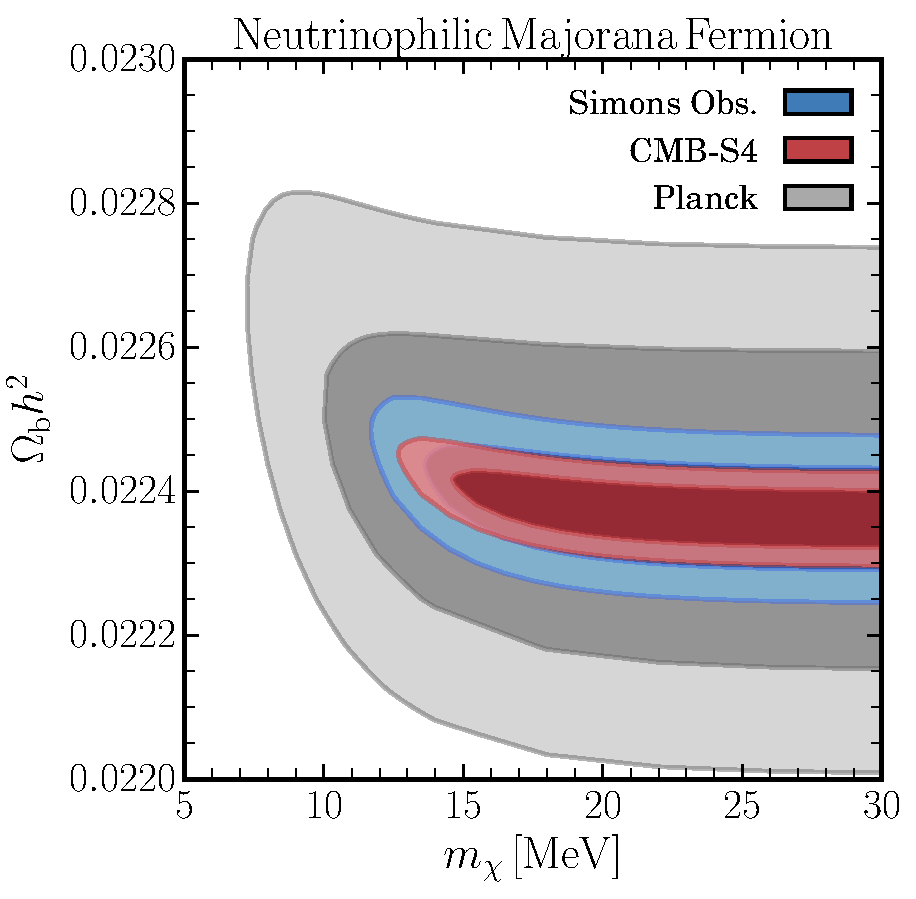
\includegraphics[width=0.45\textwidth,height=200pt]{figures/Nu_Maj_cmb_exclusion.pdf} \qquad
    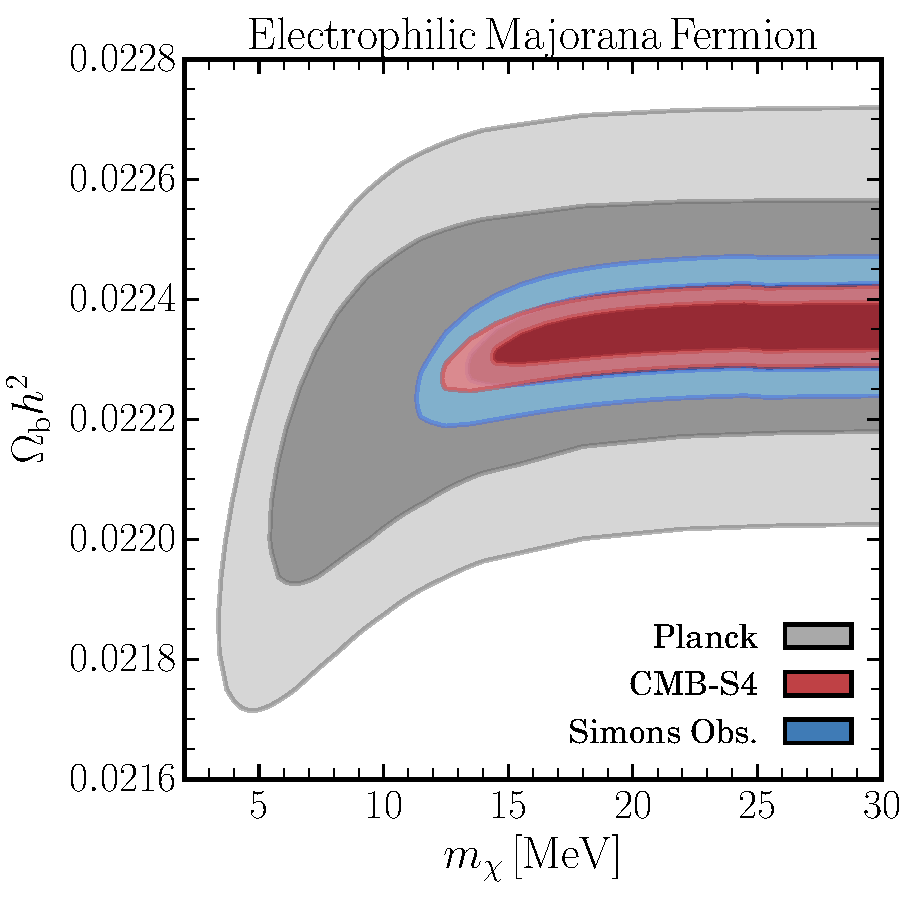
\includegraphics[width=0.45\textwidth,height=200pt]{figures/EE_Maj_cmb_exclusion.pdf}
    \caption{Contour plots showing the current and forecasted $1\sigma$ and $2\sigma$ confidence intervals in the $(\Omega_{\mathrm{b}} h^2$,\,$m_\chi)$ plane for a BSM Majorana fermion in thermal equilibrium with the SM plasma during BBN. The grey contours correspond to current constraints by Planck 2018, while the blue and red contours correspond to the expected reach of the Simons Observatory and CMB-S4 experiments respectively. \emph{Left}: Neutrinophilic. \emph{Right}: Electrophilic.}
    \label{fig:Future_1-2D}
\end{figure*}


%%%%%%%%%%%%%%%%%%%%%%%%%%%%%%%%%%%%%%%%%%%%%%%%%%%%%%
\subsection{Cosmic Microwave Background}\label{sec:future_CMB}
%%%%%%%%%%%%%%%%%%%%%%%%%%%%%%%%%%%%%%%%%%%%%%%%%%%%%%
There are a number of proposed future CMB experiments that would provide an accurate determination of the relevant cosmological parameters for this study: $\Omega_{\mathrm{b}} h^2,\,N_{\rm eff},\,Y_{\rm P}$. Proposed experiments include satellite missions like PICO~\cite{Hanany:2019lle} or CORE~\cite{DiValentino:2016foa} and ground-based experiments like the Simons Observatory~\cite{Ade:2018sbj}, CMB-S4~\cite{Abazajian:2016yjj,Abazajian:2019eic} and CMB-HD~\cite{Sehgal:2019ewc}. In this section we consider the reach of the Simons Observatory\footnote{\url{https://simonsobservatory.org/}.}, because it is fully funded and expected to deliver measurements within the next few years, and that of CMB-S4\footnote{\url{https://cmb-s4.org/}.}, because it aims to reach a sub-percent determination of $N_{\rm eff}$.

We use the Fisher Matrix method to forecast the reach of CMB-S4 (see Appendix~\ref{app:CMBfisher} for details) and use the baseline covariance matrix from the Simons Observatory collaboration. In analogy with~\eqref{eq:chi2_CMB}, the relevant parameters read:

\begin{center}
\resizebox{0.49\textwidth}{!}{
\begin{minipage}{0.5\textwidth}
\centering \textit{Simons Observatory}
\begin{align}
(\Omega_{\mathrm{b}} h^2,\,N_{\rm eff},\,Y_{\rm P})|_{\rm Fiducial} &= (0.022360,\, 3.046,\, 0.2472) \, \nonumber, \\
(\sigma_{1},\,\sigma_{2},\,\sigma_{3}) &= (0.000073,\, \,\,\,0.11,\, 0.0066)\, , \nonumber \\
(\rho_{12},\,\rho_{13},\,\rho_{23}) &= (0.072,\, 0.33,\, -0.86) \, ,\nonumber
\end{align}
\end{minipage}}
\resizebox{0.49\textwidth}{!}{
\begin{minipage}{0.5\textwidth}
\centering \textit{CMB-S4}
\begin{align}
(\Omega_{\mathrm{b}} h^2,\,N_{\rm eff},\,Y_{\rm P})|_{\rm Fiducial} &= (0.022360,\, 3.046,\, 0.2472) \, , \nonumber  \\
(\sigma_{1},\,\sigma_{2},\,\sigma_{3}) &= (0.000047,\, 0.081,\, 0.0043)\,  ,\nonumber\\ 
(\rho_{12},\,\rho_{13},\,\rho_{23}) &= (0.25,\, 0.22,\, -0.84) \, ,\nonumber
\end{align}
\end{minipage}}
\end{center}
Note that the forecasted errors on $N_{\rm eff}$ look substantially larger than what is typically quoted in the literature and this is simply a result of the fact we also allow $Y_{\rm P}$ to vary.

Figure~\ref{fig:Future_1-2D} shows the reach of future CMB observations to $m_\chi$ and $\Omega_{\rm b}h^2$ for a Majorana fermion. From Table \ref{tab:analysis_summary}, we notice that future CMB experiments will be able to probe substantially heavier BSM states than current CMB observations. In particular, the Simons Observatory is expected to set a lower bound on the mass of light BSM species of $m_\chi > 9.4$ MeV, while CMB-S4 is expected to extend this bound to $m_\chi > 10.5$ MeV, both at 95.4\% CL.


%%%%%%%%%%%%%%%%%%%%%%%%%%%%%%%%%%%%%%%%%%%%%%%%%%%%%%
\subsection{Big Bang Nucleosynthesis}\label{sec:future_BBN}
%%%%%%%%%%%%%%%%%%%%%%%%%%%%%%%%%%%%%%%%%%%%%%%%%%%%%%

Forecasting the reach of future determinations of the light primordial element abundances is not straightforward. However, from an observational perspective, the precision with which the primordial deuterium abundance is measured, is expected to improve by an order of magnitude with upcoming 30 m telescope facilities~\cite{Cooke:2016rky,Grohs:2019cae}. From a theoretical perspective, the nuclear reaction rates that significantly contribute to the error budget in the theoretical prediction of ${\rm D/H}|_{\rm P}$ are expected to be measured with higher accuracy by the LUNA collaboration~\cite{Trezzi:2018qjs}. It is therefore feasible that, in the near future, a per mille determination of ${\rm D/H}|_{\rm P}$ could be achieved. Regarding $Y_{\rm P}$, while the situation is much less clear, it is still conceivable that $Y_{\rm P}$ could be narrowed down with greater than $1\,\%$ accuracy in the future~\cite{Grohs:2019cae}.

In order to account for many possible future scenarios, and in a similar spirit to \cite{Lague:2019yvs}, we estimate the reach of future measurements of $Y_{\rm P}$ and ${\rm D/H}|_{\rm P}$ to the mass of thermal BSM state by assuming that the measured values of $Y_{\rm P}$ and ${\rm D/H}|_{\rm P}$ correspond to the values as predicted by \texttt{PRIMAT} using $\Omega_{\mathrm{b}} h^2 = 0.02236$ and $\tau_n = 879.5$ s -- namely, $Y_{\rm P} = 0.2472$ and ${\rm D/H}|_{\rm P} = 2.439 \times 10^{-5}$ -- and by varying the joint theoretical + observational accuracy with which they are determined.

In Figure~\ref{fig:futureBBN}, we show the forecasted $2\sigma$ lower bounds on the mass of a Majorana fermion in thermal equilibrium with the SM plasma as a function of the fractional error in $Y_{\rm P}$ and ${\rm D/H}|_{\rm P}$. It is clear that the bounds are largely driven by helium measurements, while ${\rm D/H}|_{\rm P}$ measurements are instead expected to provide accurate determinations of $\Omega_{\mathrm{b}}h^2$. As such, if a prior for $\Omega_{\mathrm{b}}h^2$ is provided from CMB observations, then ${\rm D/H}|_{\rm P}$ measurements do play an important role in constraining light BSM species in thermal equilibrium with the SM plasma. 
\clearpage
 
\begin{figure*}[t]
    \centering
    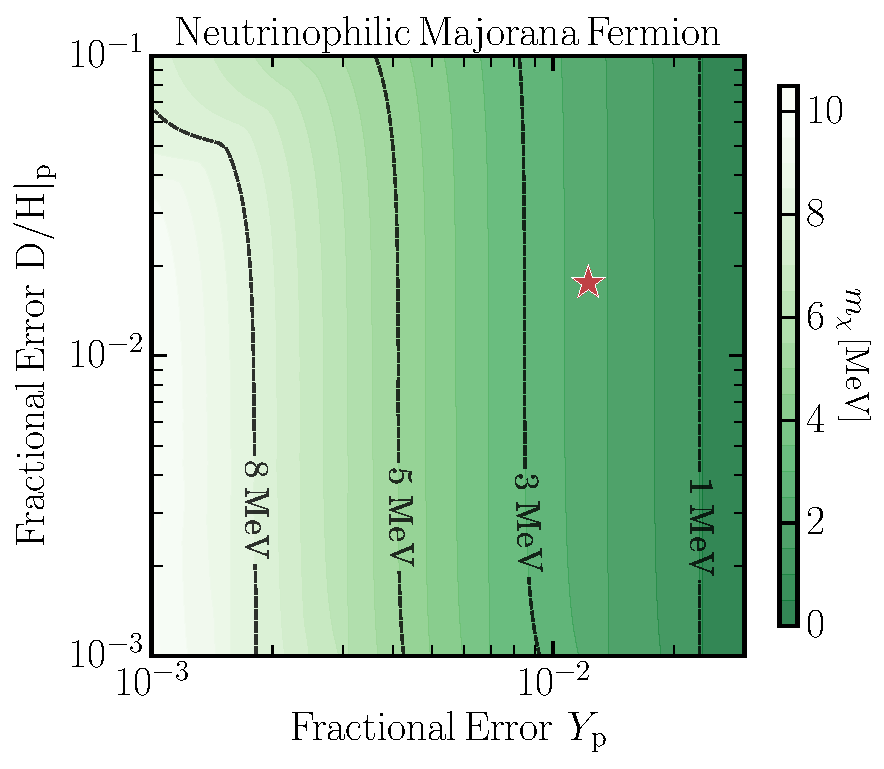
\includegraphics[width=0.7\textwidth]{figures/Nu_Maj_Errors_Levels.pdf} \\
    \quad 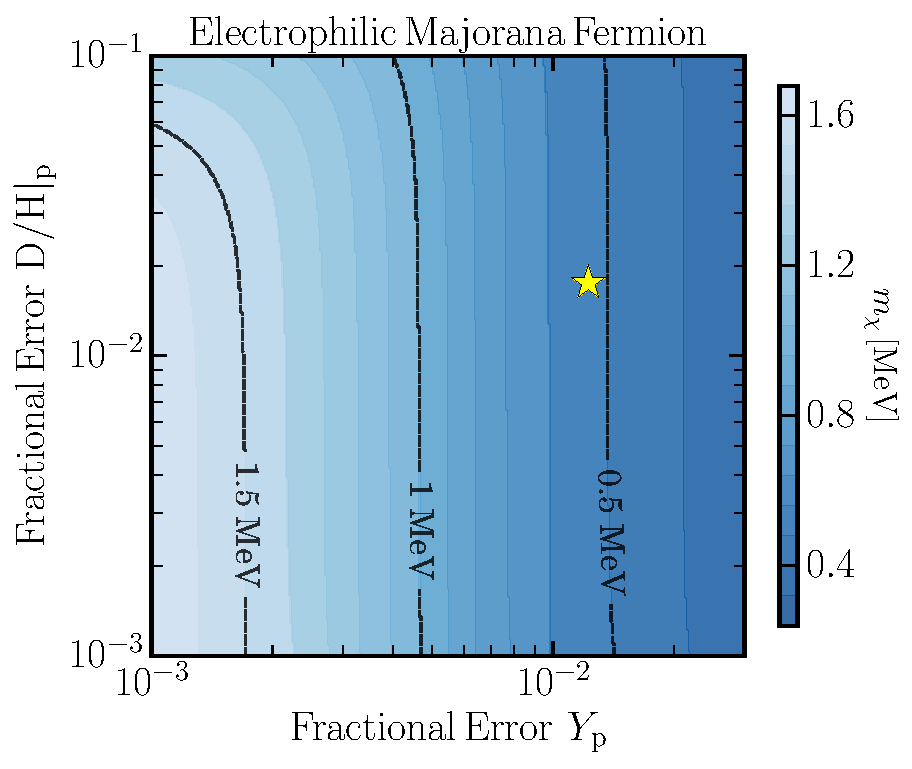
\includegraphics[width=0.72\textwidth]{figures/EE_Maj_Errors_Levels.pdf} 
    \caption{Projected $2\sigma$ exclusion limits for the mass of a Majorana BSM particle in thermal equilibrium during BBN. Bounds are shown as a function of the fractional errors (joint theoretical and observational) in the primordial helium and deuterium abundances. The red and yellow stars correspond to the current precision. \emph{Top}: Neutrinophilic. \emph{Bottom}: Electrophilic.}
    \label{fig:futureBBN}
\end{figure*}
\clearpage


%%%%%%%%%%%%%%%%%%%%%%%%%%%%%%%%%%%%%%%%%%%%%%%%%%%%%%
\section{Discussion}\label{sec:discussion}
%%%%%%%%%%%%%%%%%%%%%%%%%%%%%%%%%%%%%%%%%%%%%%%%%%%%%%
In this section we comment on some of the implications of the constraints on thermal BSM species derived in this work. In particular, we discuss examples of theoretical scenarios in which these bounds are relevant, how the bounds are altered when additional BSM states are present and the robustness of our constraints with respect to non-standard expansion histories of the Universe. Finally, we provide a brief comparison with recent literature. 
%%%%%%%%%%%%%%%%%%%%%%%%%%%%%%%%%%%%%%%%%%%%%%%%%%%%%%
\subsection{Particle Physics Scenarios} 
%%%%%%%%%%%%%%%%%%%%%%%%%%%%%%%%%%%%%%%%%%%%%%%%%%%%%%

Our constraints on thermally coupled BSM species apply to various particle physics models, typically within the context of thermal dark matter. The bounds outlined in Table~\ref{tab:DMbounds} apply to both s-wave and p-wave annihilating thermal relics. Such bounds are particularly relevant for s-wave and p-wave dark matter particles annihilating to neutrinos~\cite{Boehm:2006mi,Farzan:2009ji,Farzan:2011ck,Batell:2017cmf,Ballett:2019cqp}, since they are difficult to test at neutrino experiments \cite{Kamada:2015era,Arguelles:2017atb,Alvey:2019jzx,Klop:2018ltd,Kelly:2019wow}. In addition, these bounds will  be relevant for p-wave annihilating relics to electrons and positrons, as in the case of Majorana/Dirac dark matter annihilating via dark photon/Higgs exchange \cite{Krnjaic:2015mbs,Alexander:2016aln,Battaglieri:2017aum,Beacham:2019nyx}. Furthermore, the bounds apply to species that need not to be the entirety of the dark matter, see e.g.~\cite{Berlin:2018sjs}, and have also been applied to scenarios in which dark matter particles interact with  quarks~\cite{Krnjaic:2019dzc}. 

The bounds derived in \cite{Sabti:2019mhn} for BSM species that annihilate into electrons and neutrinos with different ratios are, for instance, relevant for scenarios involving a gauging of SM global symmetries such as $U(1)_{L_\mu-L_\tau}$ \cite{Arcadi:2018tly,Kamada:2018zxi,Foldenauer:2018zrz} or $U(1)_{B-L}$ \cite{Okada:2010wd,Escudero:2018fwn}. Finally, these bounds also apply to asymmetric dark matter sectors interacting with SM species~\cite{Zurek:2013wia,Petraki:2013wwa}. Asymmetric dark matter set-ups require annihilation cross sections that are larger than for WIMPs, and as such thermal equilibrium in the early Universe is realised. Note, however, that these bounds do not apply to scenarios in which the given BSM species is never brought into thermal equilibrium, as in the case of freeze-in \cite{Hall:2009bx,Dvorkin:2019zdi}, or simply for significantly smaller couplings than those outlined in Equations \eqref{eq:Annihilation} and \eqref{eq:Decay}~\cite{Berlin:2017ftj}. For slightly smaller couplings than those in Equations \eqref{eq:Annihilation} and \eqref{eq:Decay}, BBN can still serve as a useful probe~\cite{Berlin:2019pbq}.

The bounds presented in this study do not only apply to dark matter particles, but also to unstable mediators. For example, the bounds constrain relevant parameter spaces for various neutrinophilic scalars and vector bosons, regardless of whether they are related to dark matter \cite{Blennow:2019fhy,Kelly:2019wow} or not \cite{Blinov:2019gcj}. Similarly, light dark Higgses or dark photons are also constrained. The constraints are particularly relevant for dark photons that decay into hidden sector species. Specifically, the bounds rule out MeV-scale dark photons that decay invisibly for kinetic mixing parameters in the range $10^{-7} \lesssim \epsilon \lesssim 10^{-5}$. This region of parameter space is mildly constrained from colliders, beam dump experiments and supernova cooling~\cite{Ilten:2018crw,Bauer:2018onh,Chang:2018rso}. 

%%%%%%%%%%%%%%%%%%%%%%%%%%%%%%%%%%%%%%%%%%%%%%%%%%%%%%
\subsection{Modified Cosmological Histories} 
%%%%%%%%%%%%%%%%%%%%%%%%%%%%%%%%%%%%%%%%%%%%%%%%%%%%%%

The bounds derived above were obtained assuming that only one particle alters the usual SM picture of a radiation dominated Universe between neutrino decoupling and recombination. Here we comment on how we expect the constraints to be altered when additional BSM species are present or non-standard thermal histories are considered.  

Typically, dark matter particles are accompanied with mediators of similar mass. The presence of two (or more) neutrinophilic/electrophilic particles in thermal equilibrium in the early Universe would result in stronger bounds on the individual masses of the particles as compared to those outlined in Table \ref{tab:DMbounds}. Another very plausible contribution to the energy density in the Universe during BBN and recombination is massless dark radiation adding to $\Delta N_{\rm eff}$. Massless dark radiation will contribute to the expansion rate of the Universe and hence lead to an enhancement of $Y_{\rm P}$ with respect to the SM prediction \cite{Sarkar:1995dd,Iocco:2008va,Pospelov:2010hj}. This is precisely the same effect as the light BSM particles we consider (see middle panels of Figure \ref{fig:Cosmoimply}) and hence the BBN bounds should simply strengthen in such a scenario. The CMB constraints on the other hand, will be relaxed in the case of electrophilic particles \cite{Steigman:2013yua} but strengthen for neutrinophilic species. Similarly, perhaps a more exotic non-negligible primordial leptonic asymmetry could be present and modify nucleosynthesis and $N_{\rm eff}$ as relevant for CMB observations \cite{Dolgov:2002wy}. In such a scenario, we expect the bounds presented here to be modified \cite{Berezhiani:2012ru} but not substantially given the accuracy with which $N_{\rm eff}$ and the helium and deuterium abundances have now been measured.

One of the key assumptions to derive the bounds in this study was that the particles we consider must have been in thermal equilibrium. Since we know from both BBN and CMB observations that the Universe should have at least reached a temperature of $T > 1.8\,\text{MeV}$ \cite{deSalas:2015glj,Hasegawa:2019jsa}, the particles we consider will indeed have reached thermal equilibrium. 

Another assumption in order to derive these bounds is that the baryon-to-photon ratio remains constant between the end of BBN and recombination. This is well justified on the basis that late time electromagnetic energy injections are strongly constrained by BBN \cite{Kawasaki:2017bqm,Hufnagel:2018bjp,Forestell:2018txr} and CMB spectral distortions \cite{Hu:1992dc,Hu:1993gc}.

\subsection{Comparison with Previous Literature} 

The cosmological implications of MeV-scale thermal dark matter particles were highlighted a while ago in~\cite{Kolb:1986nf}. Since then, a number of groups~\cite{Kolb:1986nf,Serpico:2004nm,Boehm:2013jpa,Nollett:2013pwa,Nollett:2014lwa,Boehm:2012gr,Ho:2012ug,Wilkinson:2016gsy,Depta:2019lbe,Escudero:2018mvt} have used BBN and/or CMB observations to set constraints on the masses and properties of various thermally coupled species in the early Universe. 

One of the main differences between previous studies and the one presented here is the accuracy with which the primordial element abundances have been calculated. In particular, we account for non-instantaneous neutrino decoupling in the presence of light BSM particles~\cite{Escudero:2018mvt,Escudero:2019new} and we use the state-of-the-art BBN code \texttt{PRIMAT}~\cite{Pitrou:2018cgg}. With respect to previous CMB analyses, we find very similar results to those presented in~\cite{Escudero:2018mvt} that accounted for the same effects and used Planck 2018 data. Regarding BBN constraints, we can differentiate between two types of studies: some that fixed the baryon-to-photon ratio to be the best-fit from CMB observations at the time \cite{Serpico:2004nm,Boehm:2013jpa,Boehm:2012gr,Depta:2019lbe}, while others allowed $\Omega_{\rm b}h^2$ to vary and then fitted it to measurements of $Y_{\rm P}$ and ${\rm D/H}|_{\rm P}$ simultaneously with $m_\chi$~\cite{Nollett:2013pwa,Nollett:2014lwa,Wilkinson:2016gsy}. In this work, we marginalize over all possible values of $\Omega_{\rm b}h^2$. The comparison with each reference goes as follows: firstly, when comparing with~\cite{Nollett:2013pwa}, we find that the constraints presented in this work on purely electrophilic BSM states are a factor $1.5-2.5$ more stringent. Secondly, a direct comparison with~\cite{Nollett:2014lwa} is not possible since there are no bounds reported from a BBN only analysis. Thirdly, \cite{Wilkinson:2016gsy} did not found a BBN bound for a real neutrinophilic scalar boson at 95.4\% CL while we find $m_\chi > 1.2\,\text{MeV}$ at such CL. We believe that these differences with previous studies are largely driven by the use of more recent and precise determinations of $Y_{\rm P}$ and ${\rm D/H}|_{\rm P}$.


%%%%%%%%%%%%%%%%%%%%%%%%%%%%%%%%%%%%%%%%%%%%%%%%%%%%%%
\section{Conclusions}\label{sec:conclusions}
%%%%%%%%%%%%%%%%%%%%%%%%%%%%%%%%%%%%%%%%%%%%%%%%%%%%%%

MeV-scale BSM species in thermal equilibrium with the Standard Model plasma during Big Bang Nucleosynthesis have important cosmological consequences, as can be seen from Figure \ref{fig:Cosmoimply}. In this work, we have analyzed in detail and with precision the impact of such states on the synthesis of the primordial element abundances and CMB observations. To this end, we have modelled the early Universe evolution using the methods of \cite{Escudero:2018mvt,Escudero:2019new} and by modifying the state-of-the-art BBN code \texttt{PRIMAT}~\cite{Pitrou:2018cgg}. We have used a suite of cosmological observations, as summarized in Table~\ref{tab:analysis_summary}, to set constraints on the masses of various types of BSM states in thermal equilibrium with the SM plasma during BBN. We summarize the derived constraints in Table~\ref{tab:DMbounds} for purely electrophilic and neutrinophilic BSM states. The main conclusions that can be drawn from this study are:
 
\begin{itemize}[leftmargin=0.6cm,itemsep=2pt] 
\item BBN observations set a lower bound on electrophilic/neutrinophilic thermal species of $m_\chi > 0.4/1.2 \,\text{MeV}$ at 95.4\% CL. This bound is independent of the spin and the number of internal degrees of freedom of the species at hand. In particular, any WIMP, irrespective of its annihilation being s-wave or p-wave and the annihilation final state, is bounded to have $m_\chi > 0.4\,\text{MeV}$ at 95.4\% CL.


\item Very light ($m_\chi < 0.1\,\text{MeV}$) thermal relics are highly disfavoured by current measurements of the primordial light elements (at more than $5\sigma$). The sole exception to this rule is a purely neutrinophilic neutral scalar state, which is nonetheless ruled out at $3.3\sigma$. 

\item BBN and CMB observations jointly constrain neutrinophilic and electrophilic thermal BSM states to have a mass $m_\chi > 3.7\,\text{MeV}$ at 95.4\% CL. This bound is independent of the spin or internal degrees of freedom of the given species and applies to both s-wave and p-wave annihilating dark matter relics, as well as to unstable dark sector mediators. Table \ref{tab:DMbounds} summarizes the constraints for various BSM states.

\item We argue that the bounds presented in this study are expected to be strengthened in the presence of additional species beyond those considered here. In addition, bounds based on BBN are largely insensitive to modifications of the assumed cosmological model.

\item In \cite{Sabti:2019mhn}, there are also constraints set on BSM particles with masses $m_\chi \lesssim 20 \,\text{MeV}$ that interact with both electrons and neutrinos. Such states efficiently delay the process of neutrino decoupling, which allows BBN to constrain the temperature of neutrino decoupling to be $T_{\nu} ^{\rm dec} > 0.34\,\text{MeV}$ at 95.4\% CL. Moreover, we find that decoupling temperatures $T_{\nu} ^{\rm dec} < 0.2 \,\text{MeV}$ are highly disfavoured ($> 5\sigma$) by BBN and/or CMB observations.

\item Future CMB experiments such as the Simons Observatory~\cite{Ade:2018sbj} and CMB-S4~\cite{Abazajian:2016yjj,Abazajian:2019eic}, will constrain generic thermal BSM particles of $m_\chi \lesssim (10-15)\,\text{MeV}$. Similarly, we highlighted the impact of future primordial helium and deuterium determinations to light BSM states in thermal equilibrium with the SM plasma during nucleosynthesis. 
\end{itemize}


\noindent To summarize, cosmology strongly constrains new physics at the MeV scale. Cosmological constraints are competitive with and complementary to those from  colliders, beam dump and neutrino experiments, (in)direct dark matter searches, as well as from astrophysical probes. 